\documentclass[10pt]{article}
\usepackage{amsmath} 
\usepackage{fontspec}
\usepackage[a4paper, margin=12mm]{geometry}
\usepackage{graphicx}
\usepackage{titlesec}
\usepackage{amsmath}
\usepackage{fancyhdr}
\usepackage{amsmath}
\usepackage{datetime}
\usepackage[hidelinks]{hyperref}
\usepackage[utf8]{inputenc}
\usepackage{enumitem}
\usepackage{booktabs}
\usepackage{pifont}

\setmainfont{JetBrains Mono}
\setmainfont[NFSSFamily=dayrom]{JetBrains Mono}
\graphicspath{ {./images/} }

\DeclareSymbolFont{digits}{TU}{dayrom}{m}{n}
\AtBeginDocument{
	\DeclareMathSymbol{0}{\mathalpha}{digits}{`0}
	\DeclareMathSymbol{1}{\mathalpha}{digits}{`1}
	\DeclareMathSymbol{2}{\mathalpha}{digits}{`2}
	\DeclareMathSymbol{3}{\mathalpha}{digits}{`3}
	\DeclareMathSymbol{4}{\mathalpha}{digits}{`4}
	\DeclareMathSymbol{5}{\mathalpha}{digits}{`5}
	\DeclareMathSymbol{6}{\mathalpha}{digits}{`6}
	\DeclareMathSymbol{7}{\mathalpha}{digits}{`7}
	\DeclareMathSymbol{8}{\mathalpha}{digits}{`8}
	\DeclareMathSymbol{9}{\mathalpha}{digits}{`9}
}

% subsubsubsection
\titleclass{\subsubsubsection}{straight}[\subsection]
\newcounter{subsubsubsection}[subsubsection]
\renewcommand\thesubsubsubsection{\thesubsubsection.\arabic{subsubsubsection}}
\renewcommand\theparagraph{\thesubsubsubsection.\arabic{paragraph}} % optional; useful if paragraphs are to be numbered
\newcommand{\cmark}{\ding{51}} % Haken
\newcommand{\xmark}{\ding{55}} % Kreuz
\newcommand{\checkbox}{$\square$} % leere Checkbox

\titleformat{\subsubsubsection}
{\normalfont\normalsize\bfseries}{\thesubsubsubsection}{1em}{}
\titlespacing*{\subsubsubsection}
{0pt}{3.25ex plus 1ex minus .2ex}{1.5ex plus .2ex}

\makeatletter
\renewcommand\paragraph{\@startsection{paragraph}{5}{\z@}%
	{3.25ex \@plus1ex \@minus.2ex}%
	{-1em}%
	{\normalfont\normalsize\bfseries}}
\renewcommand\subparagraph{\@startsection{subparagraph}{6}{\parindent}%
	{3.25ex \@plus1ex \@minus .2ex}%
	{-1em}%
	{\normalfont\normalsize\bfseries}}
\def\toclevel@subsubsubsection{4}
\def\toclevel@paragraph{5}
%\def\toclevel@paragraph{6}
\def\toclevel@subparagraph{6}
\def\l@subsubsubsection{\@dottedtocline{4}{7em}{4.5em}}
\def\l@paragraph{\@dottedtocline{5}{10em}{5em}}
\def\l@subparagraph{\@dottedtocline{6}{14em}{6em}}
\makeatother

\setcounter{secnumdepth}{4}
\setcounter{tocdepth}{4}


\hypersetup{
	colorlinks=true,
	urlcolor=cyan,
}

% Footer-Einstellungen
\newdateformat{mydate}{\twodigit{\THEDAY}.\twodigit{\THEMONTH}.\THEYEAR}
\mydate
\pagestyle{fancy}
\fancyhf{} % Löscht alle Kopf- und Fusszeilen
\fancyfoot[C]{\thepage\ -\ \today\ \copyright\ Bastian\ Kind,\ James\ Binks,\ Mark\ Matkovic\ und\ David\ Hafner} % Setzt den Foote

\begin{document}
	\section{BandE}
	\subsection{Barrierefreiheit umsetzen}
	\subsubsection{Was ist barrierefreiheit in einer Applikation}
	Barrierefreiheit beschreibt wie einfach die Applikation gebraucht werden kann auch für personen mit einschränkungen.
	Einige Beispiele von Barrierefreiheit sind:
	\begin{itemize}
		\item Screenreader
		Eine Möglichkeit den inhalt der Applikation vorgelesen bekommen zu können. Ideal für Blinde Nutzer.
		\item Schriftgrösse verstellen
		Die verstellung der schrifftgrösse erlaubt es auch Personen mit Seheinschränkungen die Applikation problemlos zu verwenden.
		\item Einfache Sprache
		Die Sprache in der Applikation sollte simpel gehalten werden das auch junge Personen oder Personen welche sich nicht im Fachbereich auskennen den Inhalt trotzdem verstehen können.
		\item Sprachen
		Mehrere Sprachen erlauben es mehr verschiedenen Nutzer die Applikation zu verwenden.
		\item Symbole
		Symbole verwenden damit alle möglichen Personen möglichst schnell die Funktion eines Knopfes verstehen können\\\\
	\end{itemize}

	Beim entwerfen einer Applikation sollte auf die Barrierefreiheit geachtet werden, aber die Anforderungen sind nicht für alle gleich. Für eine Applikation mit der man sich für eine schwiereige English Prüfung anmelden kann, braucht nicht mehrere Sprachoptionen.\\
	Oder bei der Webseite für einen Augenoptiker lohnt es sich eine leicht verstellbare schriftgrösse zu haben.
	\subsubsection{Barrierefreiheit unserer der Applikation}
	Da unsere Applikation von alle möglichen Personen verwendet werden kann. Es sollte also simple Sprache verwenden, eine verstellbare Schriftgrösse haben und zusätzlich noch einen Screenreader haben.\\ Dies haben wir alles in den Einstellungen als Option angegeben.\\
	Die möglichkeit schnell zwischen allen 4 gängigen Landessprachen zu wechseln ist in der Navbar aufzufindne.
	Fast alles wird mit Symbolen beschrieben. Alles wird somit Intuitive gestaltet und erlaubt damit dass alle unsere App problemlos verwenden können.
	
	\subsection{Barrierefreiheit prüfen}
	\subsubsection{Wie kann Barrierefreiheit Prüfen}
	Zum Prüfen von Barrierfreihiet in Applikationen gibt es mehrere möglichkeiten.
	\begin{itemize}
		\item Automatische Tools
		\item Checklisten mit Richtlinien
		\item Nutzertest
		\item Manuelle Tests
	\end{itemize}
	Da wir keine Nutzer haben, Die Onlinetools nicht immer alles erwichen und wir keine Zeit haben alles Manuell zu testen, haben wir uns für die Checkliste mit Richtlinein entschieden.
	\subsubsection{Barrierefreiheit-Checklist}
	Aus den Rahmenbedingungen der Applikation konnten dies Checkpunkte für die Barrierefreihet herausgelesen werden.
	\begin{itemize}
		\item Alle 4 Landessprachen sollten verfügbar sein
		\item Gut Lesbare Schrift
		\item Screenreader für Seheingeschränkte
		\item Verstellbare Schriftgrösse
		\item Simple Sprache
	\end{itemize}
	\subsubsection{Benutzerschnittstelle gemäss checkliste Prüfen}
	Als Benutzerschnittstell nehmen wir die Hauptseite.
	\begin{itemize}
		\item Es gibt die möglichkeit schnell von hier zwischen den Landessprachen zu wechseln.
		\item Die Schrifft welche verwendet wird ist gut lesbar, der Rest ist mit leicht verständlichen Symbolen gestaltet.
		\item Der Screenreader ist über die Einstellungen verfügbaer und ist Standardmässig eingeschaltet
		\item Die Schriftgrösse ist über die  Einstellungen verstellbar
		\item Der Text der verwendet wird ist Simple oder wird durch Symbole Klar gemacht
	\end{itemize}
	
	\subsubsection{Barrierefreiheit Nachweisen}
	Die Barrierefreihet wurde durch das testen mit mehreren Personen Nachgewiesen. Keiner der Testpersonen hatten Probleme beim verwenden oder verstehen der Applikation.\\\\
	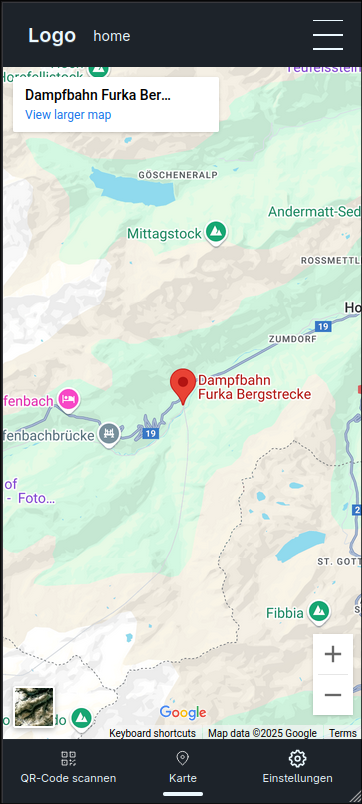
\includegraphics[width=7cm ]{mainpage}
	
\end{document}